\subsection{Bluetooth} \label{sec:bluetooth}
Another possible radio technology for presence detection is Bluetooth.
Bluetooth is a common technology used in many devices such as smartphones, tablets, and laptops.
Because it is a standardized technology, all devices that support Bluetooth can communicate with each other\cite{BluetoothOverview}.\cite{BluetoothSIG}

There are two different types of radio signals used in Bluetooth: Classic and Low Energy (LE).
They differ in terms of power consumption, range, and data transfer rate.\cite{BluetoothOverview}

\begin{figure}[h!]
  \centering
  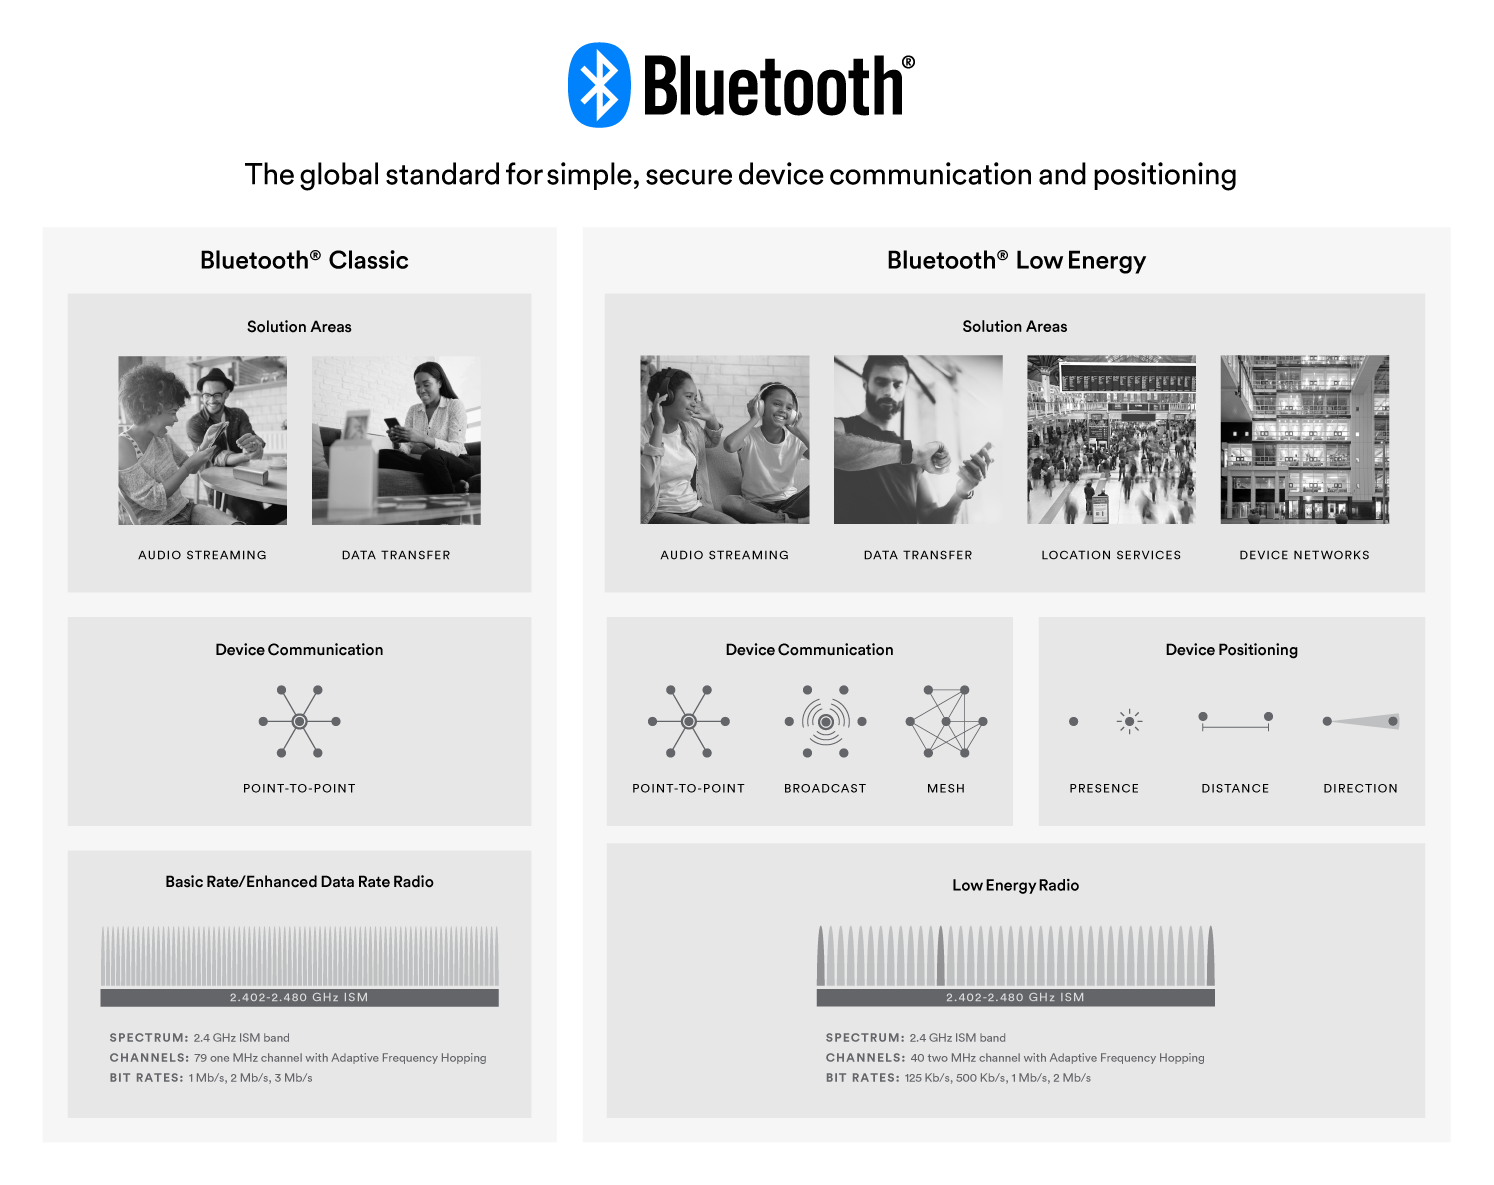
\includegraphics[width=1\textwidth]{Bluetooth_Technology_Overview_Graphic.png}
  \caption{Overview of the Bluetooth Classic and Low Energy technologies\cite{BluetoothOverview}.}
  \label{fig:classic_vs_LE}
\end{figure}

\subsubsection{Bluetooth Classic} \label{sec:bluetooth_classic}
The Bluetooth Classic radio is the original version of the Bluetooth technology introduced in 1999 for point-to-point device communication.
It is used for data transfer between devices but is primarily used for wireless audio streaming across devices because of its high data transfer rate.
According to the Bluetooth Special Interest Group (SIG), the data transfer rate of Bluetooth Classic is 3 Mb/s.\cite{BluetoothSIG}\cite{BluetoothOverview}

Wireless devices such as headphones, speakers, and car stereos often use Bluetooth Classic to stream audio to and from a smartphone.
However, the relatively high power consumption of Bluetooth Classic makes it unsuitable for presence detection using battery-powered devices.
Furthermore, it is quite sensitive to obstructions, making it less suitable for presence detection compared to Bluetooth Low Energy.\cite{BluetoothOverview}\cite{BluetoothAudioStreaming}

\subsubsection{Bluetooth Low Energy} \label{sec:bluetooth_low_energy}
Bluetooth Low Energy (BLE) is a newer version of the Bluetooth technology introduced in 2010 designed for low power consumption.
In contrast to Bluetooth Classic, the data transfer rate of BLE is much lower.
This makes it more usable in battery-powered devices such as smartphones, smartwatches, and fitness trackers.\cite{BLE_Regulatory_Aspects_Document}

The BLE specification states that the maximum data transfer rate is up to 2 Mb/s.
In practice however, is often limited to between 125 kb/s - 500 kb/s.
This is because most use cases require LE Coded PHY, a feature of BLE that improves the range and robustness of the wireless communication at the cost of a lower data transfer rate.\cite{BluetoothOverview}\cite{BLE_Regulatory_Aspects_Document}

While BLE was known for its device communication capabilities, it is now widely used as a device positioning technology due to the increasing demand for accurate indoor location services.
Since its release, BLE has evolved to include features enabling it to detect the presence, distance, and direction of nearby devices by leveraging the Received Signal Strength Indication (RSSI) of BLE.
SIG themselves recommend using BLE for presence detection in indoor environments because of its low power consumption and high accuracy.\cite{BluetoothOverview}\cite{BLE_Regulatory_Aspects_Document}

Using Bluetooth for presence detection raises some concerns with privacy, since it involves collecting and processing sensitive user data.
It is possible for unauthorized third parties to intercept Bluetooth signals, potentially exposing personal information and compromising user anonymity.
In addition, continuous tracking of individuals raises concerns regarding surveillance and the potential misuse of data by third parties. 
To mitigate these risks, it is essential to implement robust security measures, such as data encryption and anonymization.
Developers should also provide transparent privacy policies that outline data collection, storage, and usage practices.\cite{BluetoothPrivacy}\cite{BLE_Security}